\section{Event Displays and Table of High Mass Dijet Events}
\label{appEvents}

\begin{figure}[!ht]
  \begin{center}
    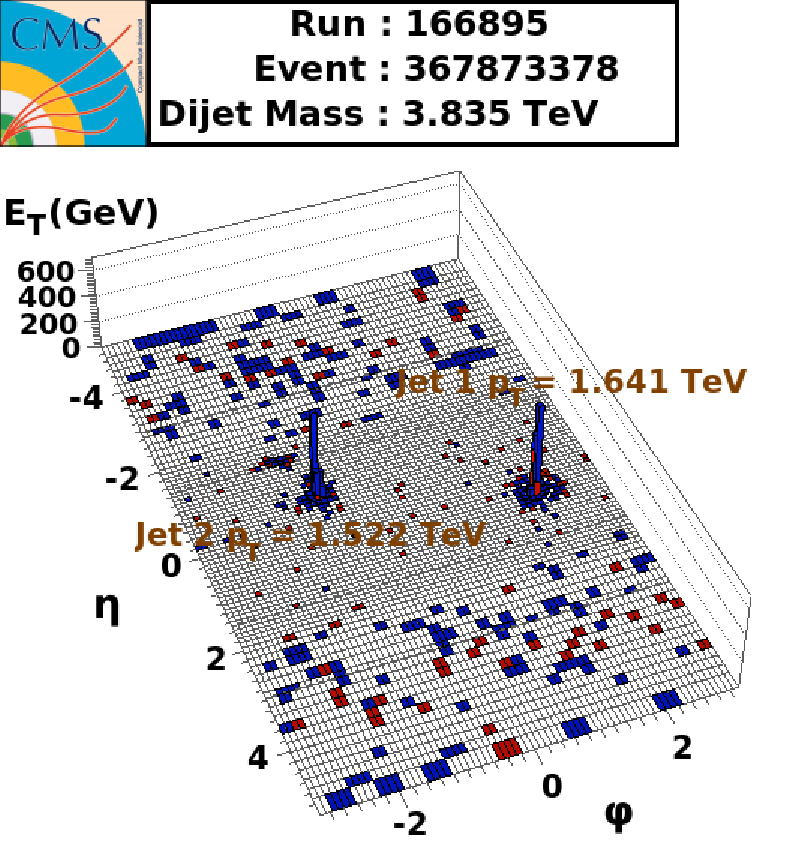
\includegraphics[width=0.37\textwidth]{Figures/EventDisplay_1st_lego.pdf}
    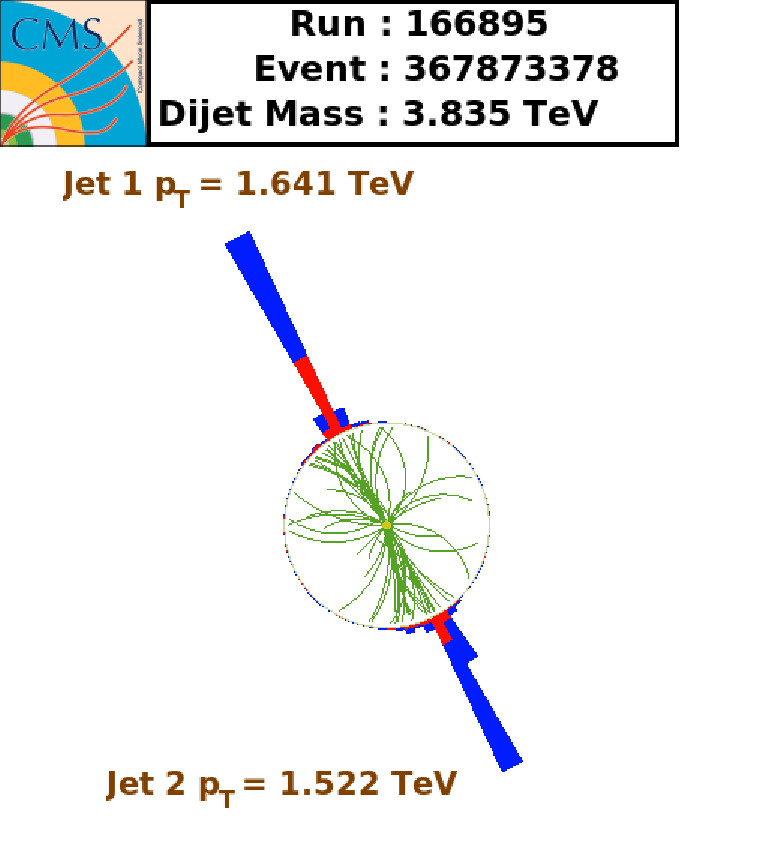
\includegraphics[width=0.37\textwidth]{Figures/EventDisplay_1st_rhophi.pdf}
    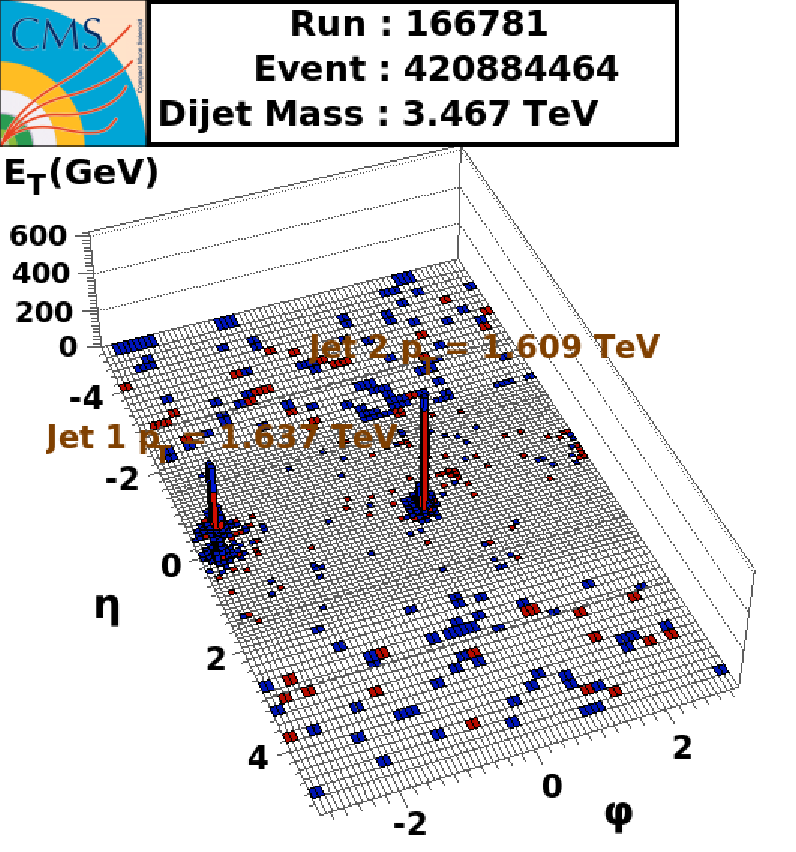
\includegraphics[width=0.37\textwidth]{Figures/EventDisplay_2nd_lego.pdf}
    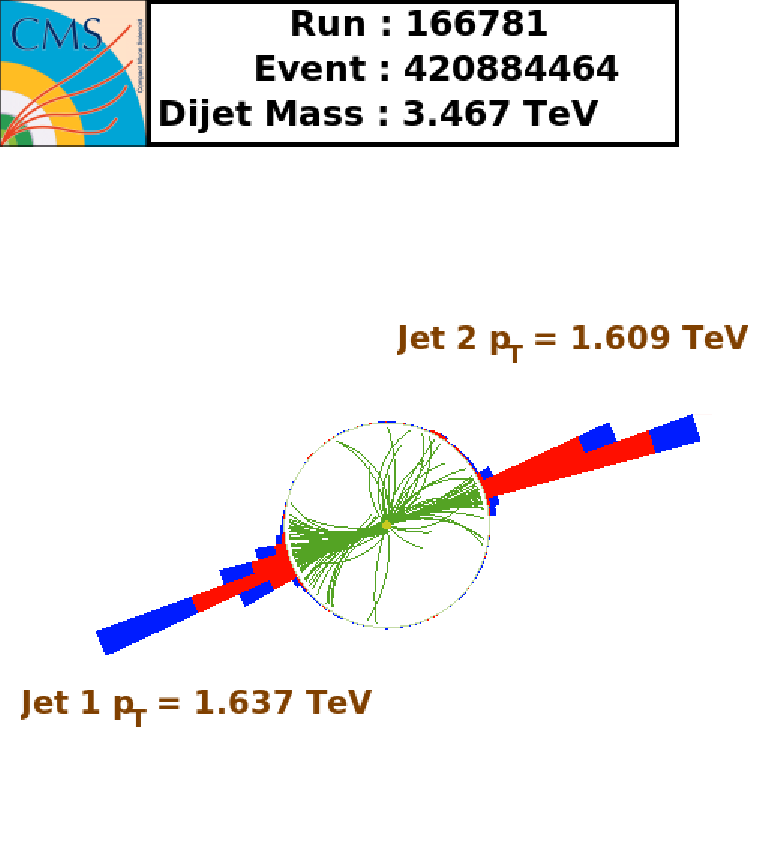
\includegraphics[width=0.37\textwidth]{Figures/EventDisplay_2nd_rhophi.pdf}
    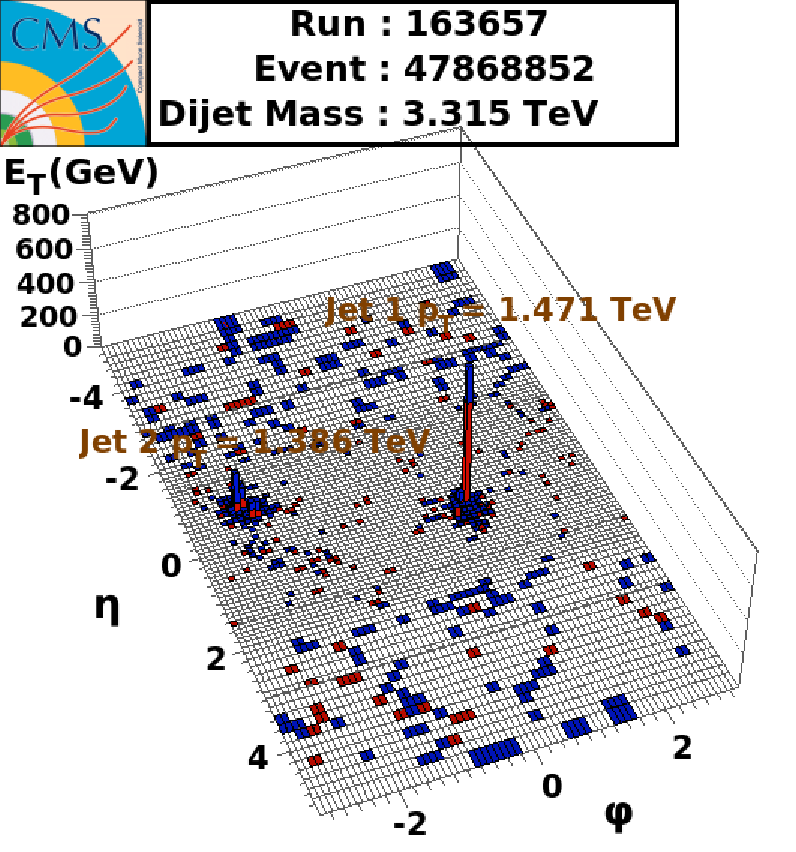
\includegraphics[width=0.37\textwidth]{Figures/EventDisplay_3rd_lego.pdf}
    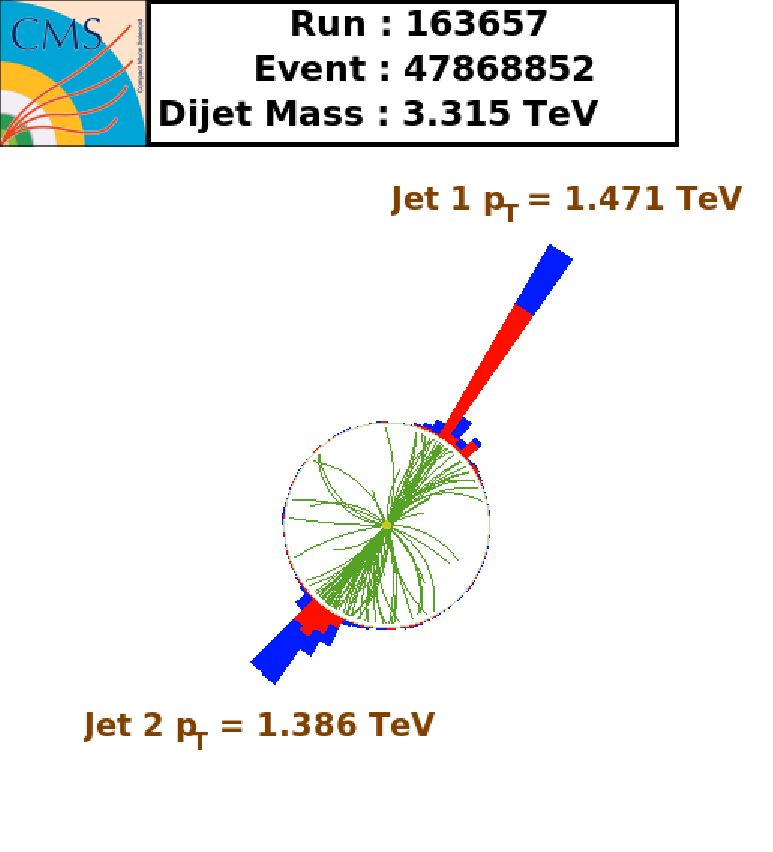
\includegraphics[width=0.37\textwidth]{Figures/EventDisplay_3rd_rhophi.pdf}
    \caption{Lego (left) and $\rho-\phi$ (right) displays of the 1st to 3rd Highest Masss Dijet Events}
    \label{MultiEventDisplay1}
  \end{center}
\end{figure}

\begin{figure}[!ht]
  \begin{center}
    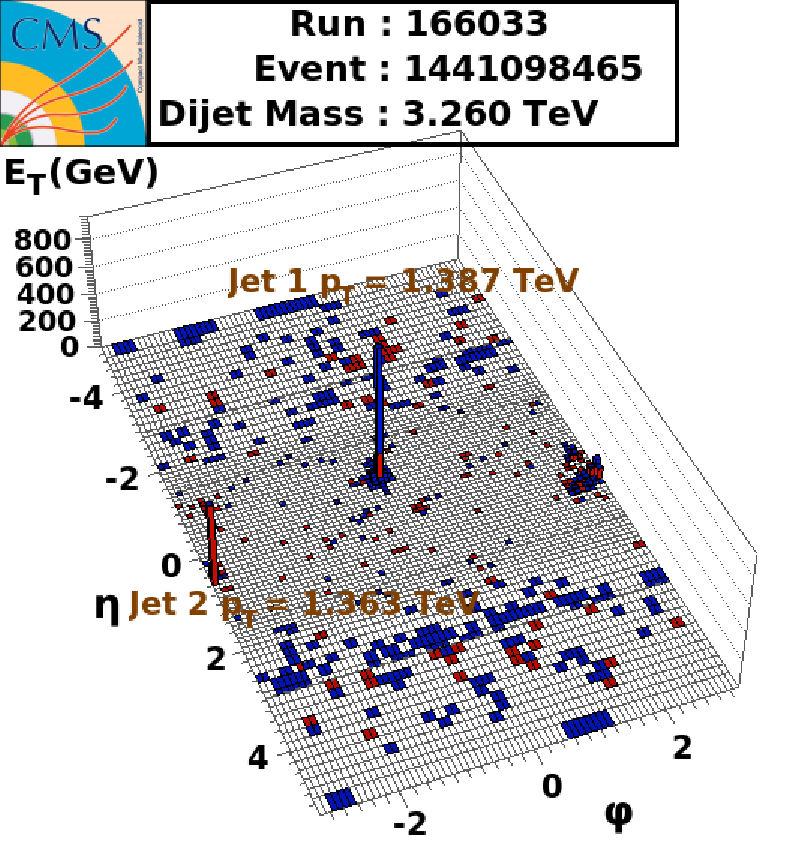
\includegraphics[width=0.42\textwidth]{Figures/EventDisplay_4th_lego.pdf}
    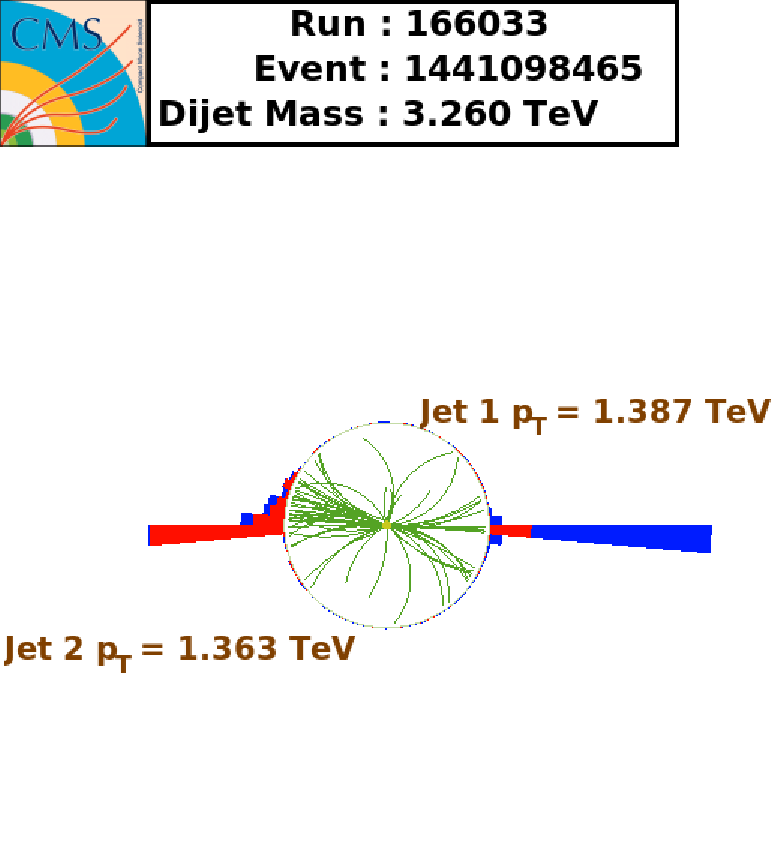
\includegraphics[width=0.42\textwidth]{Figures/EventDisplay_4th_rhophi.pdf}
    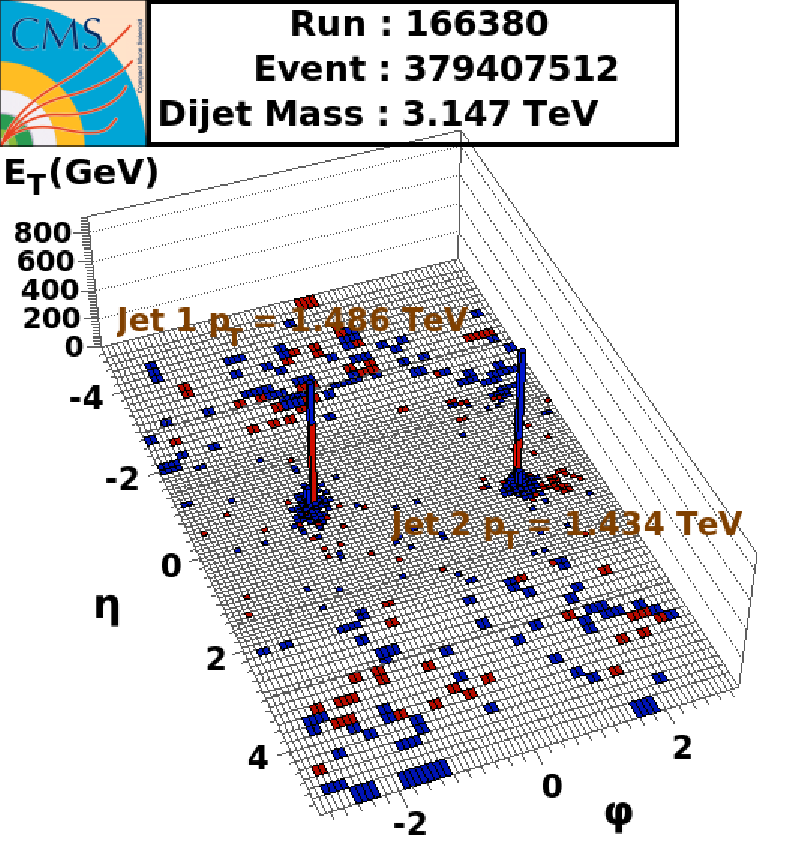
\includegraphics[width=0.42\textwidth]{Figures/EventDisplay_5th_lego.pdf}
    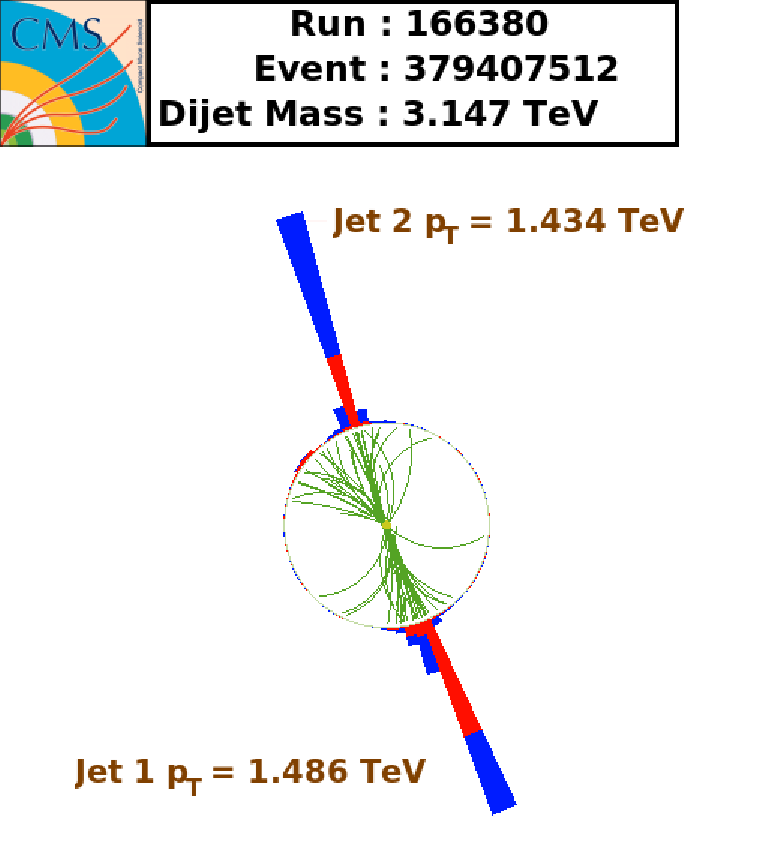
\includegraphics[width=0.42\textwidth]{Figures/EventDisplay_5th_rhophi.pdf}
    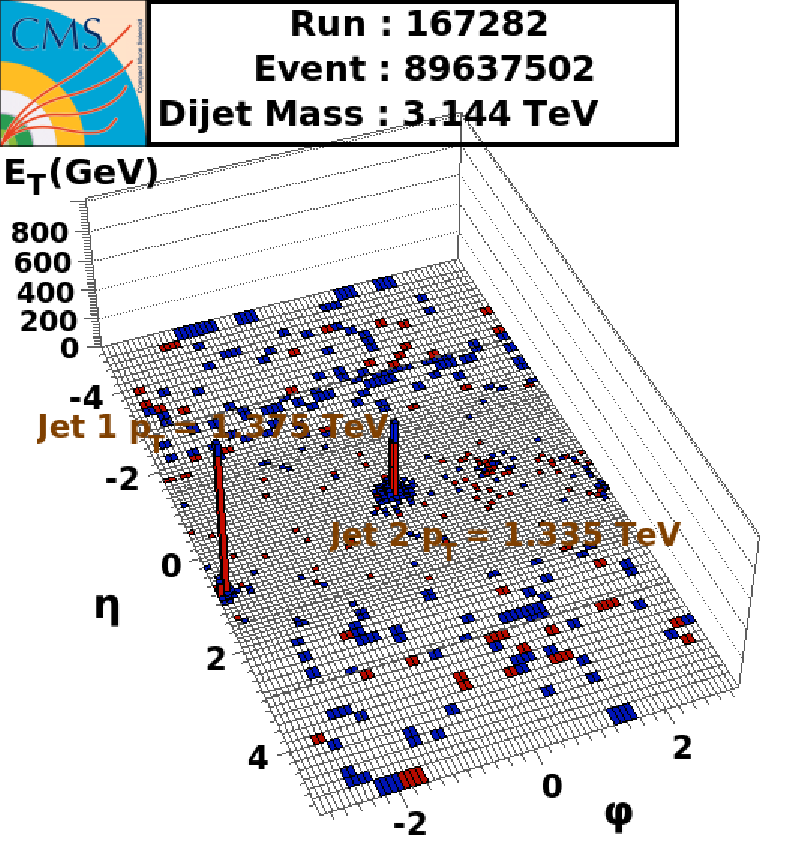
\includegraphics[width=0.42\textwidth]{Figures/EventDisplay_6th_lego.pdf}
    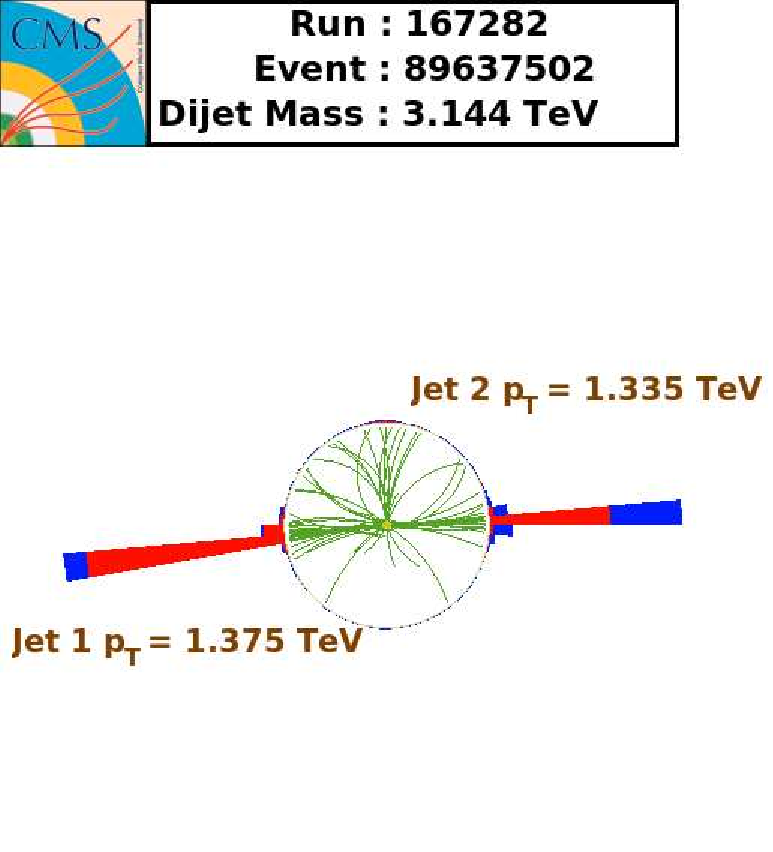
\includegraphics[width=0.42\textwidth]{Figures/EventDisplay_6th_rhophi.pdf}
    \caption{Lego (left) and $\rho-\phi$ (right) displays of the 4th to 6th Highest Masss Dijet Events}
    \label{MultiEventDisplay2}
  \end{center}
\end{figure}

\begin{figure}[!ht]
  \begin{center}
    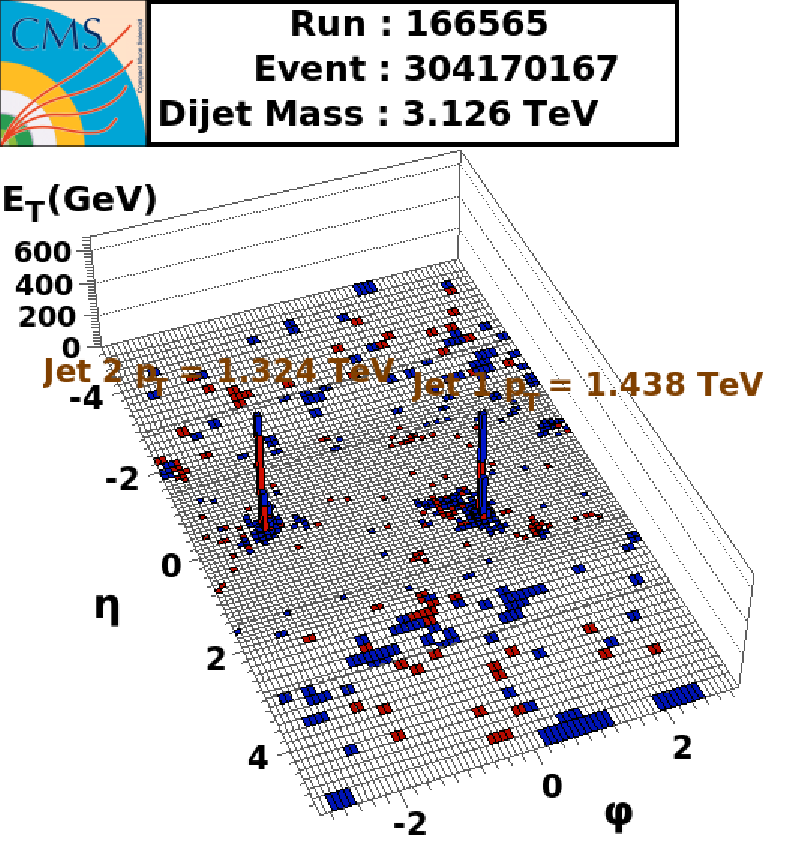
\includegraphics[width=0.31\textwidth]{Figures/EventDisplay_7th_lego.pdf}
    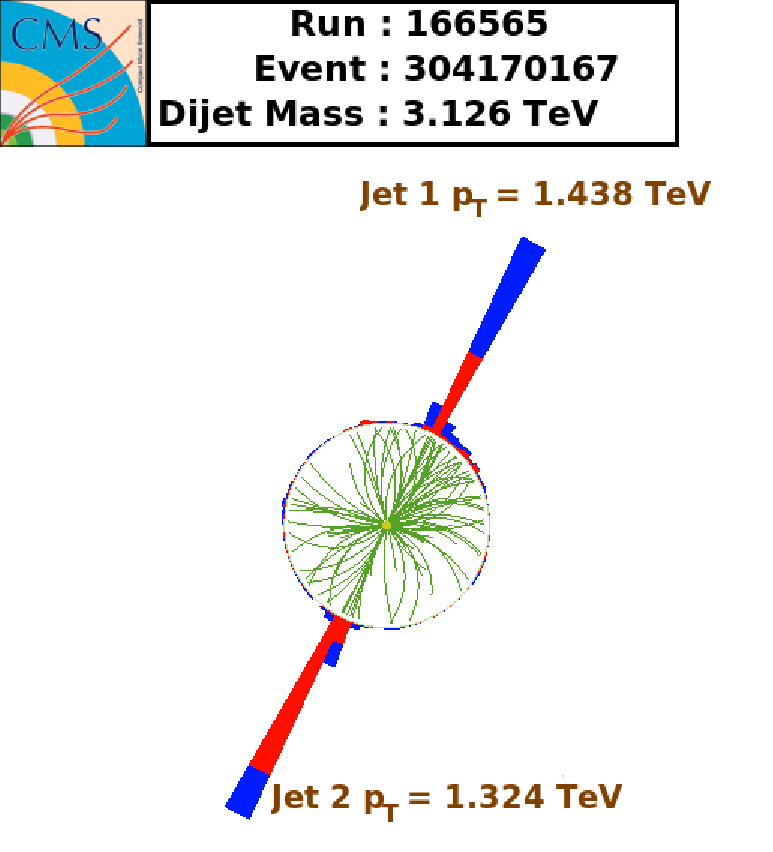
\includegraphics[width=0.31\textwidth]{Figures/EventDisplay_7th_rhophi.pdf} \\
    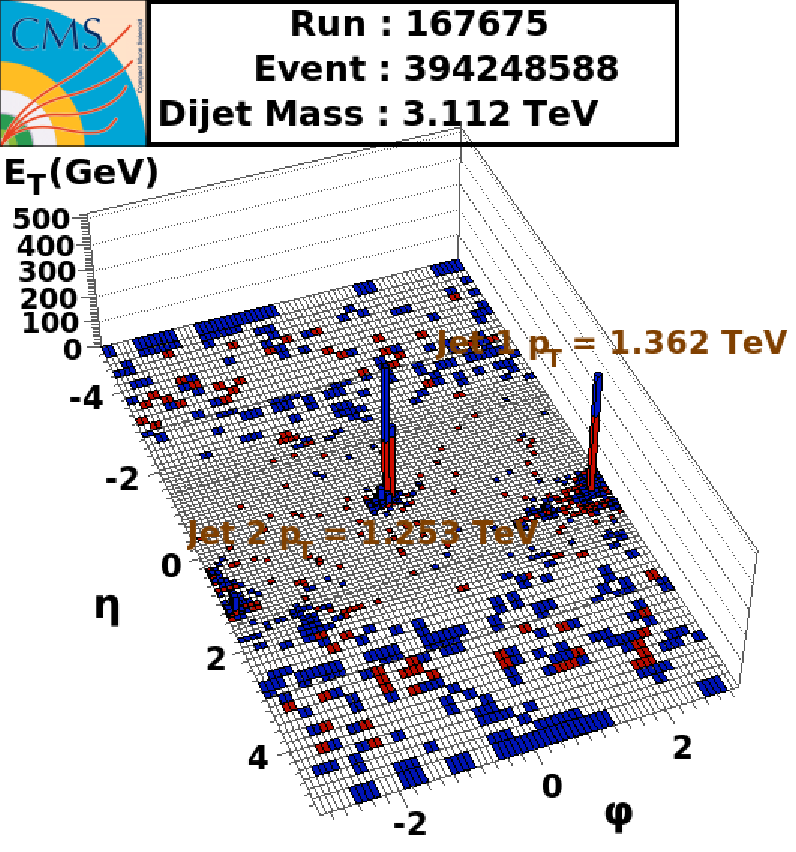
\includegraphics[width=0.31\textwidth]{Figures/EventDisplay_8th_lego.pdf}
    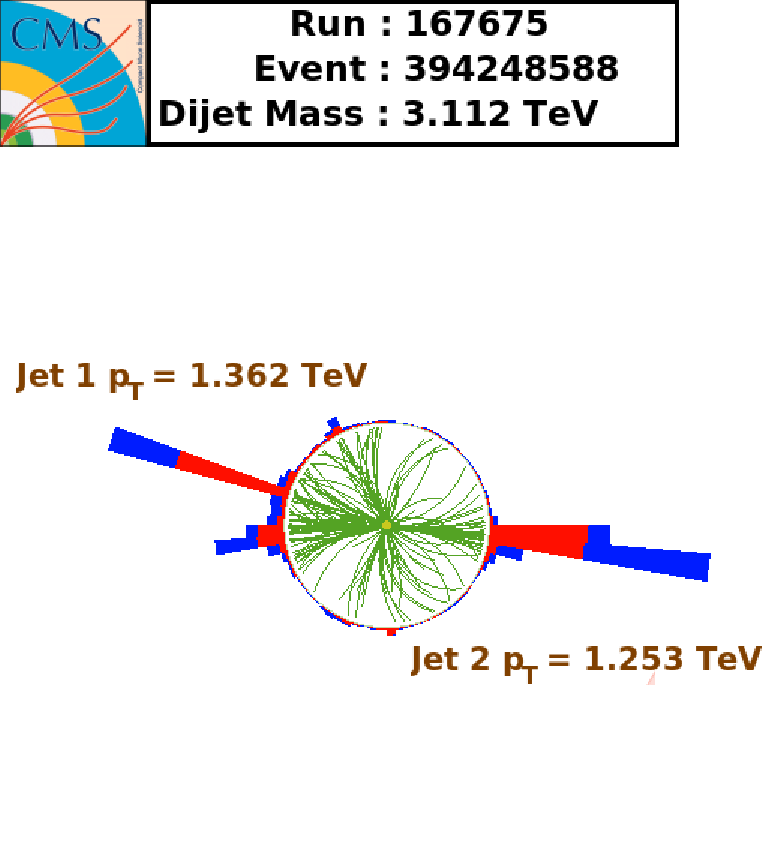
\includegraphics[width=0.31\textwidth]{Figures/EventDisplay_8th_rhophi.pdf} \\
    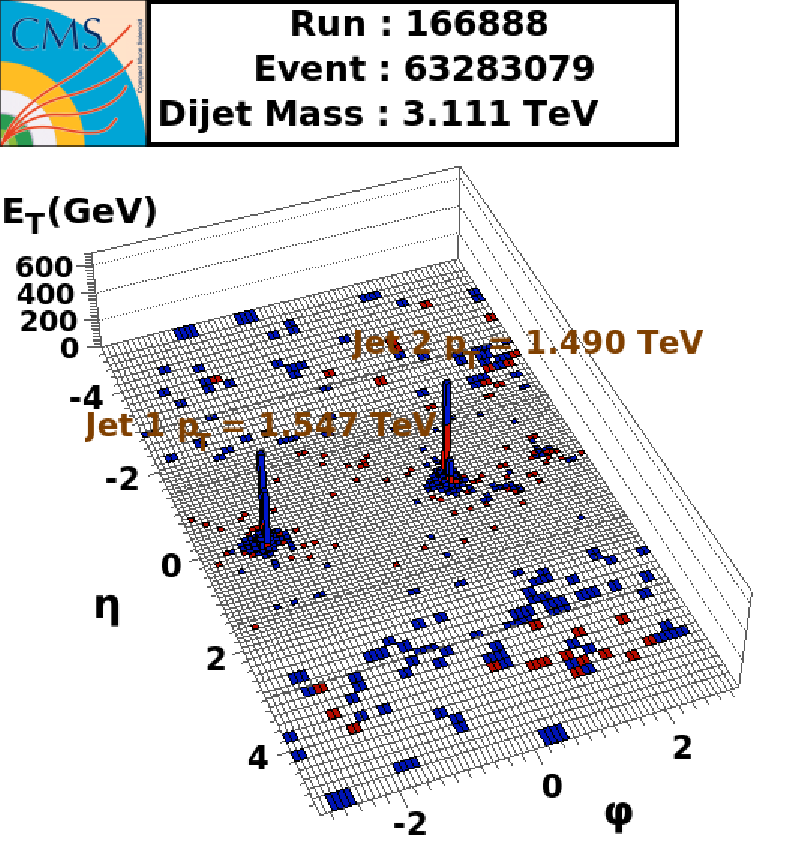
\includegraphics[width=0.31\textwidth]{Figures/EventDisplay_9th_lego.pdf}
    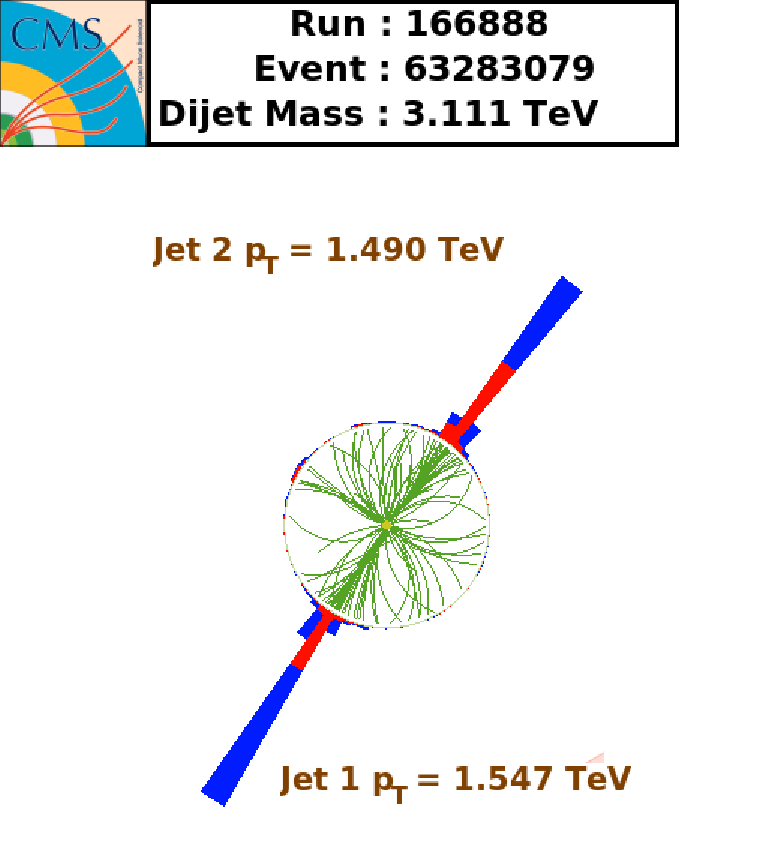
\includegraphics[width=0.31\textwidth]{Figures/EventDisplay_9th_rhophi.pdf} \\
    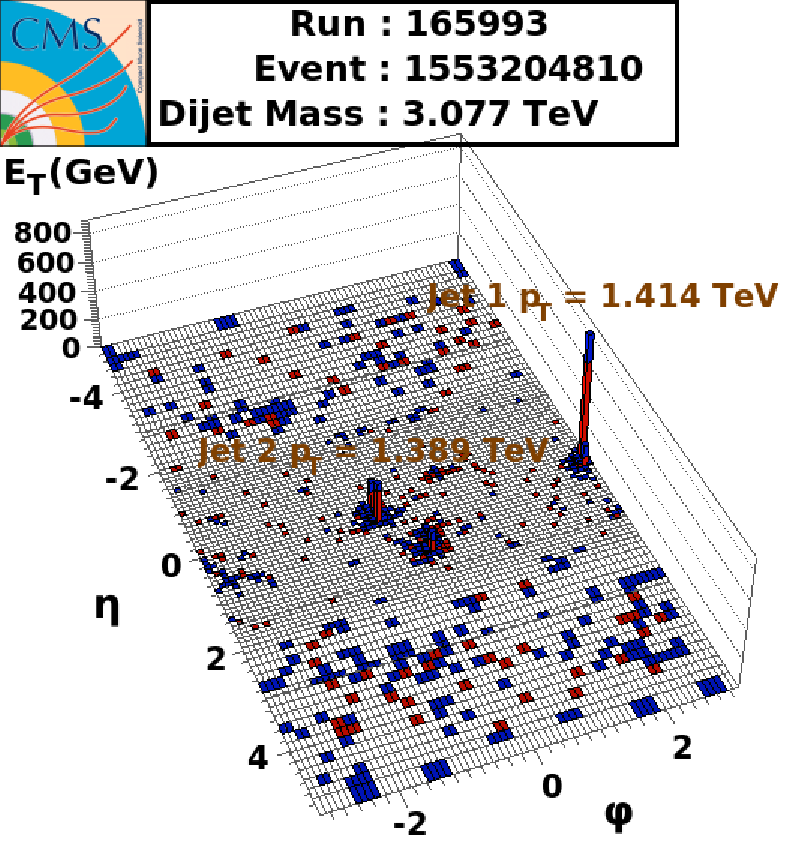
\includegraphics[width=0.31\textwidth]{Figures/EventDisplay_10th_lego.pdf}
    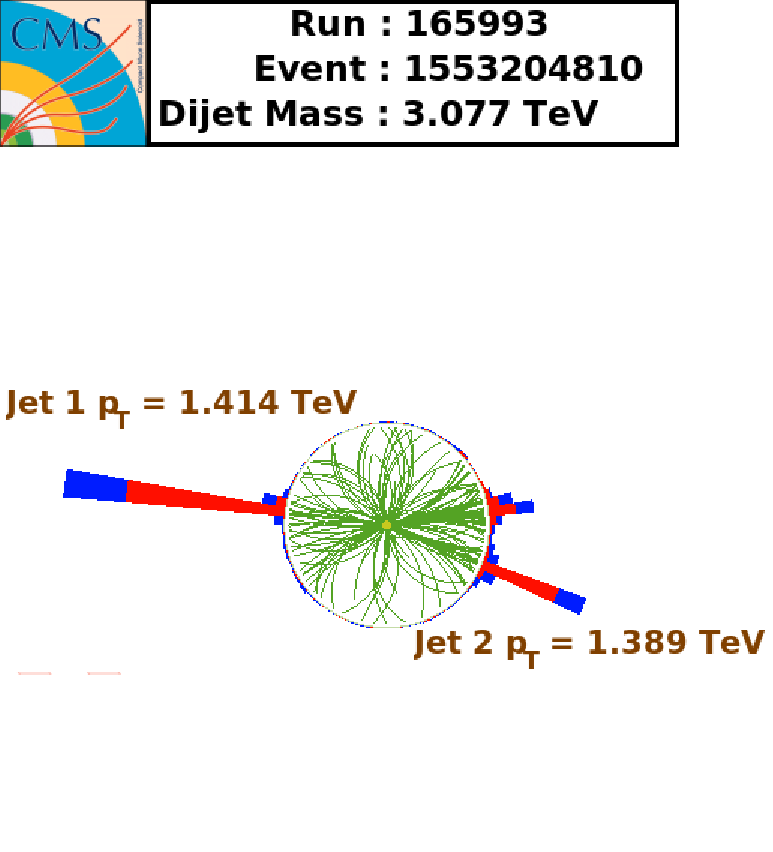
\includegraphics[width=0.31\textwidth]{Figures/EventDisplay_10th_rhophi.pdf}
    \caption{Lego (left) and $\rho-\phi$ (right) displays of the 7th to 10th Highest Masss Dijet Events}
    \label{MultiEventDisplay3}
  \end{center}
\end{figure}

\clearpage


\begin{table}[thb]
\centering
       \begin{tabular}{ |c|c||c|c|c|c|c|c|c|c| }
        \hline
        \multirow{2}{*}{$Run$} & \multirow{2}{*}{$Event$} & Dijet & $Jet$ 1   & $Jet$ 1 & $Jet$ 1  & $Jet$ 2 & $Jet$ 2 & $Jet$ 2 &  MET/$\Sigma E_T$\\
         & & Mass & Cor $p_T $ & $\eta$ & $\phi$  & Cor $p_T$ & $\eta$ & $\phi$ &  \\

          & & (TeV) & (GeV)  &  &  & (GeV) &  & &  \\
	\hline
	\hline	
	144112 & 1189490855 & 2.050 & 1099 & 0.6 & 0.1 & 935 & 0.8 & -2.8 & 0.02\\
	\hline
	142664 & 29100333 & 1.916 & 803 & -0.9 & -0.0 & 798 & 0.4 & 3.1 & 0.02\\
	\hline
	143962 & 169345756 & 1.768 & 860 & 1.5 & -2.1 & 759 & 0.7 & 1.0 & 0.06\\
	\hline
	143181 & 177895396 & 1.695 & 779 & 0.3 & 2.9 & 691 & 1.4 & -0.2 & 0.09\\
	\hline
	142528 & 201376378 & 1.642 & 743 & 0.6 & -2.4 & 687 & -0.5 & 0.8 & 0.01\\
	\hline
	144089 & 1155244569 & 1.509 & 759 & 0.2 & -2.9 & 687 & -0.3 & 0.1 & 0.06\\
	\hline
	142038 & 240422134 & 1.440 & 657 & -0.0 & 2.2 & 656 & -0.8 & -0.9 & 0.02\\
	\hline
	140383 & 191703493 & 1.413 & 599 & 0.5 & -1.4 & 568 & -0.8 & 1.7 &  0.02\\
	\hline
	142928 & 162151278 & 1.407 & 708 & 1.2 & -1.3 & 602 & 0.4 & 1.9 & 0.02\\
	\hline
	143833 & 494783908 & 1.409 & 575 & 1.2 & 0.5 & 572 & -0.1 & -2.7 & 0.05\\
	\hline

       \end{tabular}
       \caption{Dijet properties for 10 highest mass events (Leading jets corrected $p_T$, $\eta$, $\phi$, 
	 corrected Dijet Mass, and Missing ET/Sum ET).}
       \label{table_highmass2}
\end{table}
      
%\vspace*{1in}
%\begin{table}[tbh]
%\centering
%       \begin{tabular}{ |c|c||c|c|c| }
%        \hline
%        \multirow{2}{*}{$Run$} & \multirow{2}{*}{$Event$} & $Jet$ 1  & $Jet$ 2 & Dijet Mass \\
%         & & PF Cor $p_T$  & PF Cor $p_T$ & from PFJets \\
%         & & (GeV) & (GeV) & (GeV) \\
%       \hline
%        \hline
%	138919 & 32253996  & 539 & 516 & 1941 \\
%        \hline
%	139370 & 132046118 & 457 & 447 & 1374 \\
%	\hline
%	139368 & 25590516  & 610 & 609 & 1267 \\
%	\hline
%	139370 & 403257286 & 421 & 384 & 1065 \\
%	\hline
%	138921 & 16936769  & 284 & 258 & 1040 \\
%	\hline
%	139096 & 247776848 & 361 & 319 & 976 \\
%	\hline
%	139347 & 252029032 & 334 & 299 & 915 \\
%        \hline
%	139370 & 511769839 & 289 & 294 & 904 \\
%	\hline
%	139365 & 65727014  & 339 & 324 & 868 \\
%	\hline
%	138737 & 44851731  & 418 & 385 & 855 \\
%        \hline
%        \end{tabular}
%        \caption{Particle Flow Corrected $p_T$ and dijet mass of leading PF Jets matched to CaloJets for the 
%	same events as in table~\ref{table_highmass2}.  Jet 1 and 2 in this table are matched 
%	to Jet 1 and 2 in table~\ref{table_highmass2} using $\Delta R$. Note: table for the 10 highest mass 
%	dijet events in a slighly older sample, so it needs updating, but the first 4 events in this 
%	table are also in the above table and those events can be compared. }
%        \label{table_highmass3}
%\end{table}



\clearpage
